\section{Regulator \textit{swing-up}}
\subsection{Algorytm \textit{swing-up}}
Zastosowano heurystyczną regułę, która w zależności od położenia i prędkości wahadła pozwala wyznaczyć sterowanie wzbudzające system:
\begin{equation}  
u(t) = u_{swing}\cdot sgn[x_2(|x_1|-\frac{\pi}{2})]
\end{equation} 
gdzie amplituda sygnału sterującego $u_{swing} = 0.3$ wyznaczona została eksperymentalnie, tak aby położenie wózka podczas rozhuśtywania wahadła nie wykroczyło poza dopuszczalne granice. 
\subsection{Warunek przełączenia}
Algorytm \textit{swing-up} realizowany jest do momentu, kiedy do systemu zostanie dostarczona odpowiednia ilość energii, aby doprowadzić wahadło w okolice niestabilnego położenia równowagi.
Następnie sterowanie zostaje całkowicie odłączone do momentu, kiedy położenie wahadła znajdzie się w granicach $(-10^\circ,10^\circ)$. Wtedy zostaje aktywowany regulator LQR. W przypadku, kiedy stabilizacja nie powiedzie się, kąt wahadła osiągnie wartość spoza zbioru $(-30^\circ,30^\circ)$ aktywowany na nowo zostaje algorytm \textit{swing-up}. Algorytm zrealizowany został na przerzutniku RS.
\begin{figure}[H]
	\centering
	\subfloat{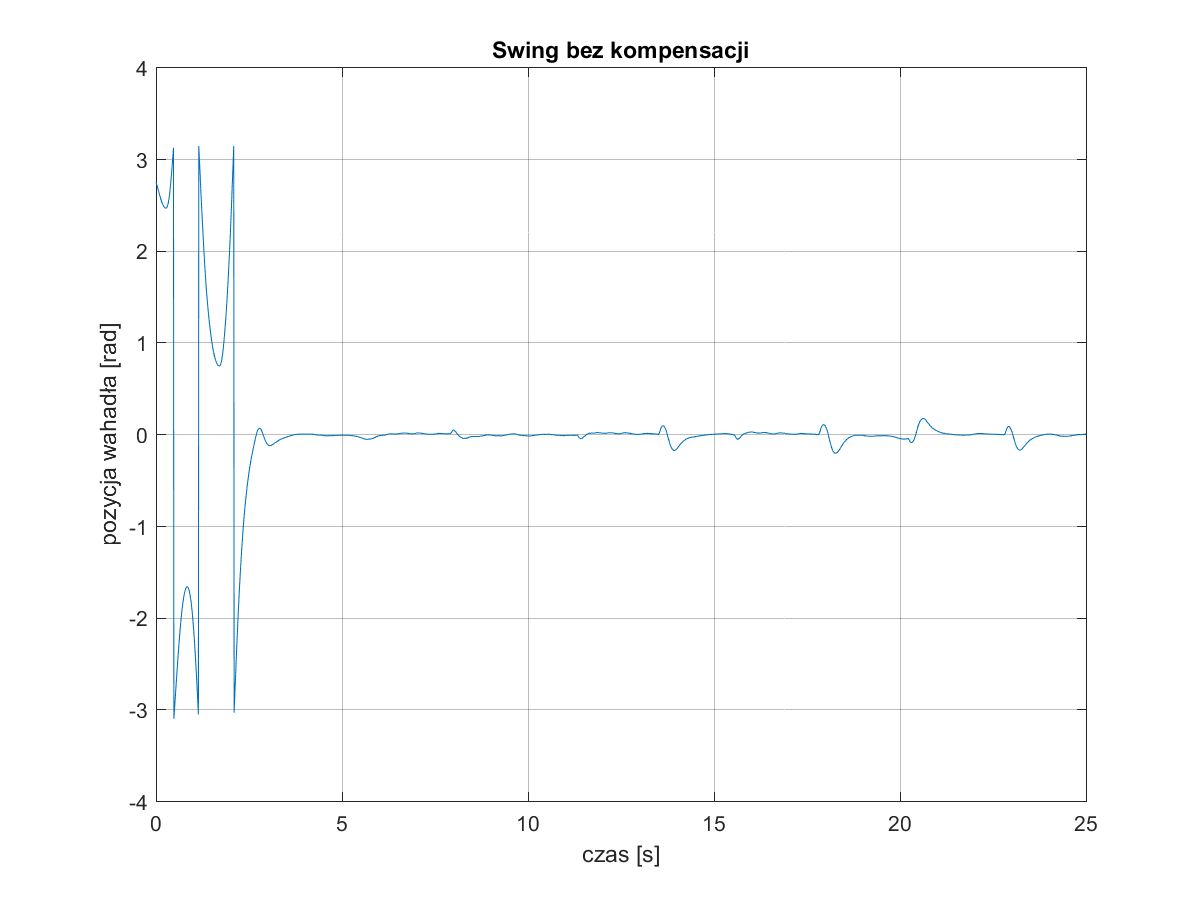
\includegraphics[width=3in]{obrazy/pendulum/Swing_bez_komp_poz_wah.png}}
	~~
	\subfloat{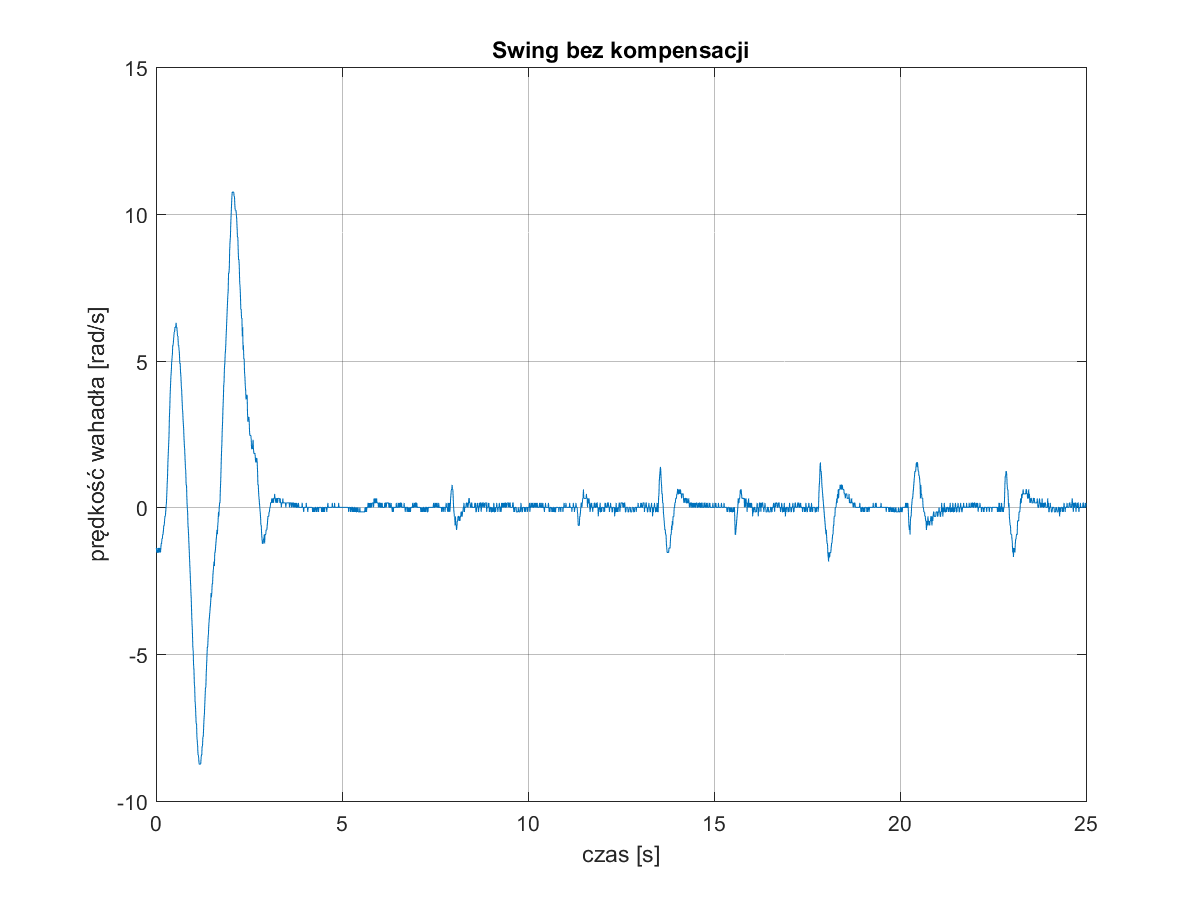
\includegraphics[width=3in]{obrazy/pendulum/Swing_bez_komp_pred_wah.png}}
	
	\subfloat{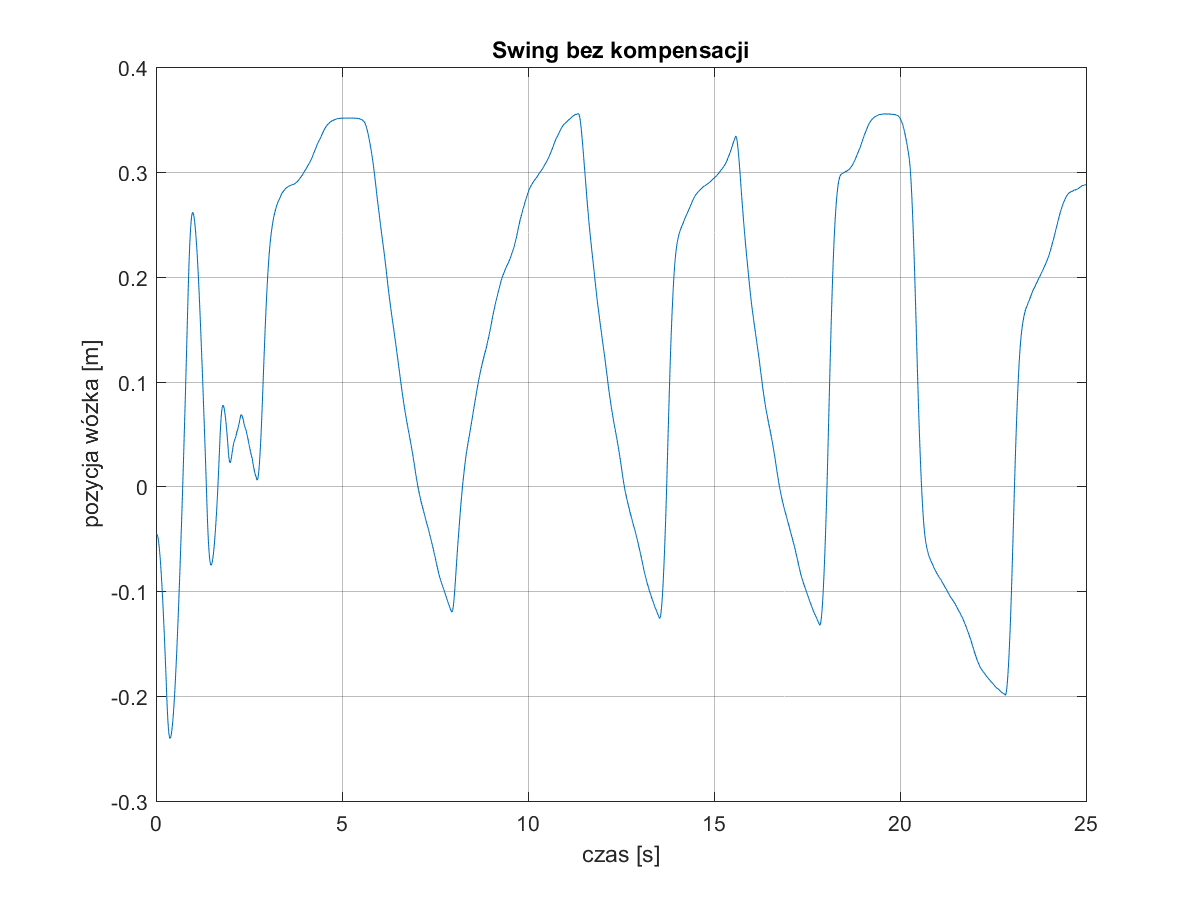
\includegraphics[width=3in]{obrazy/pendulum/Swing_bez_komp_poz_woz.png}}
	~~
	\subfloat{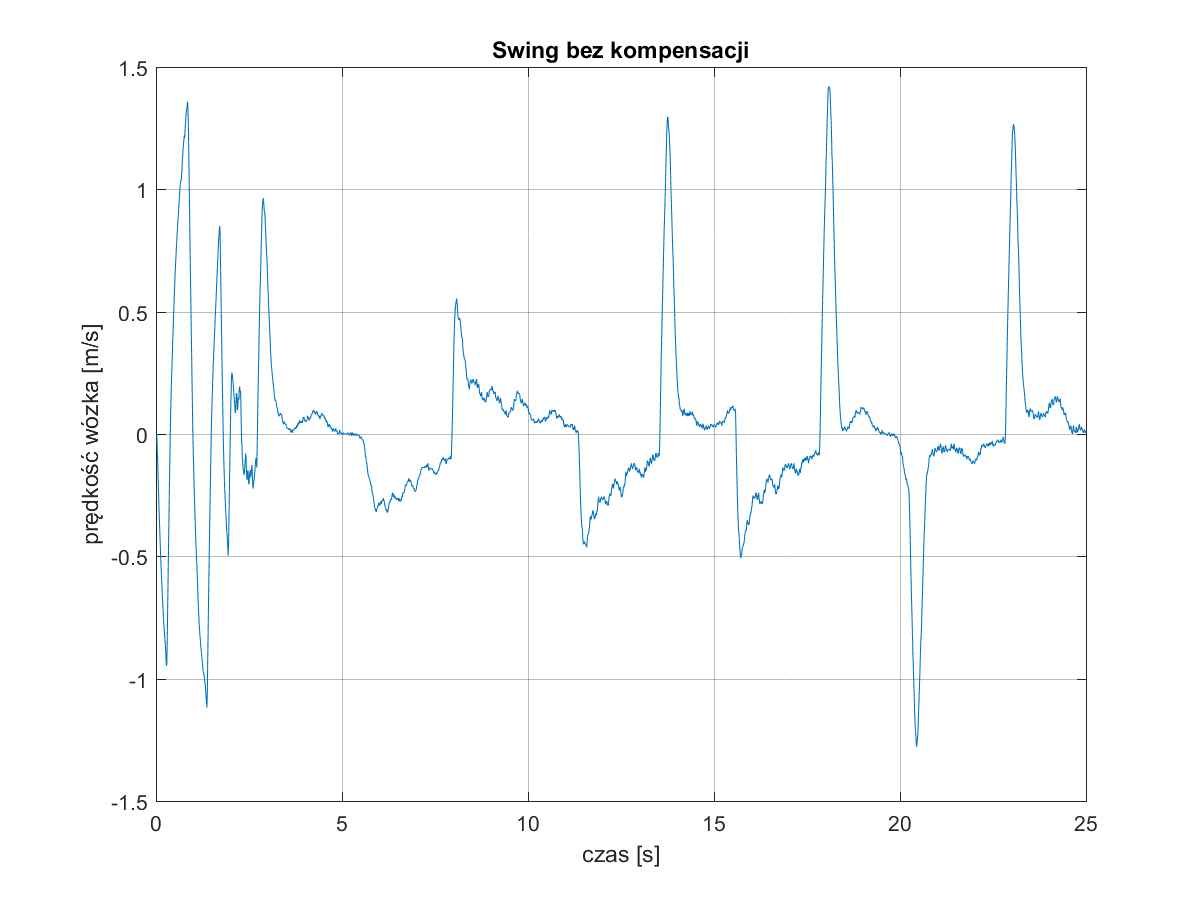
\includegraphics[width=3in]{obrazy/pendulum/Swing_bez_komp_pred_woz.png}}
	
	\subfloat{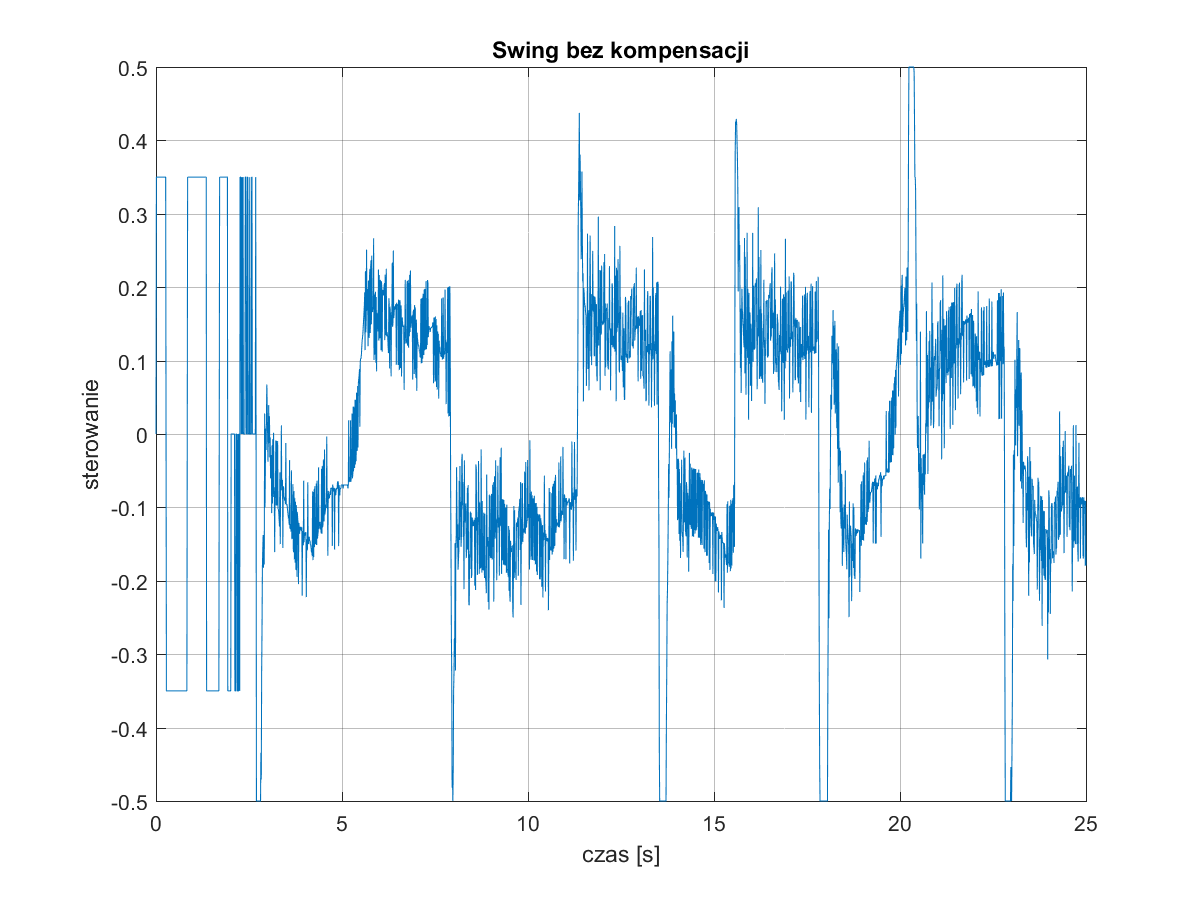
\includegraphics[width=3in]{obrazy/pendulum/Swing_bez_komp_ster.png}}
%	~~
%	\subfloat{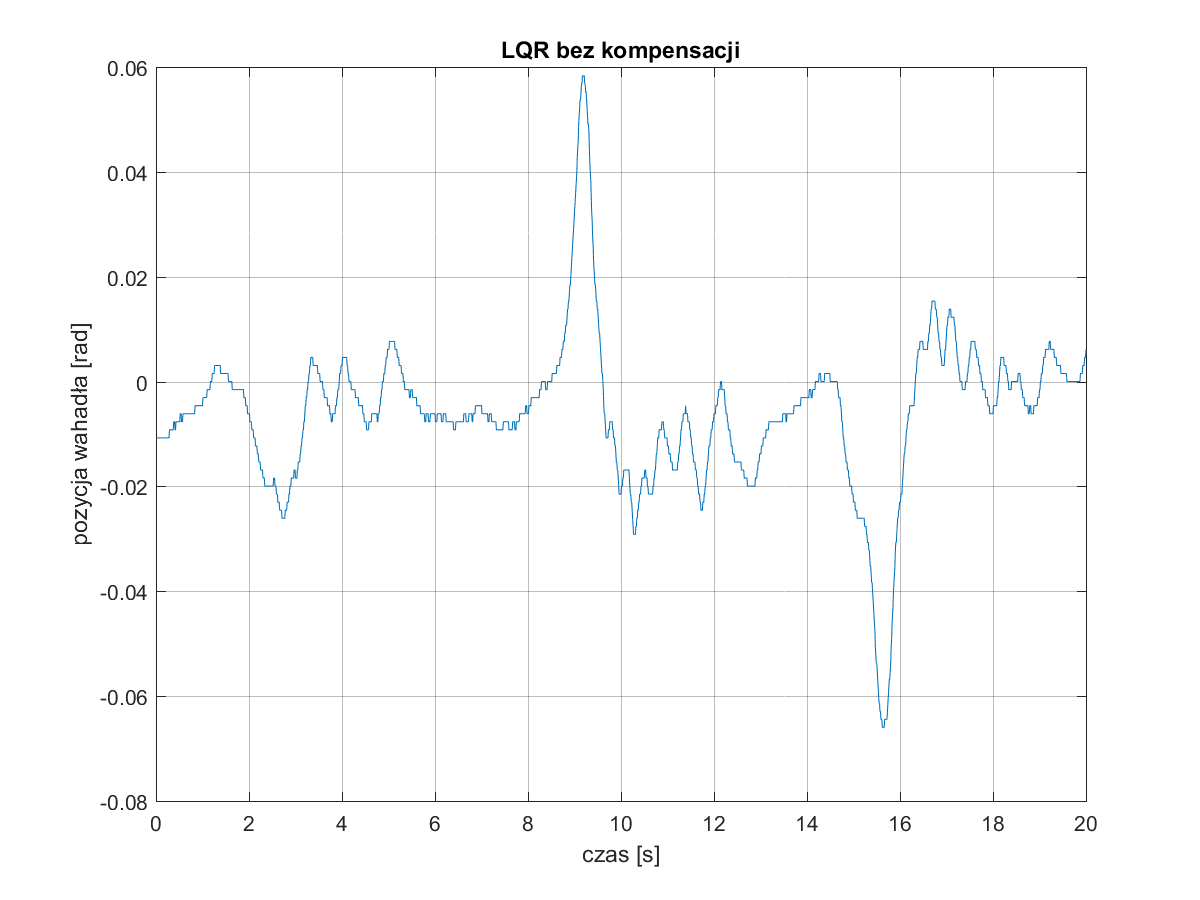
\includegraphics[width=2.8in]{obrazy/pendulum/LQR_bezk_poz_wah.png}}
	\caption{Swing-up wraz ze stabilizacją wahadła.}
\label{fig:Swing1}
\end{figure}
W celu zwiększenia skuteczności algorytmu, w momencie $t_p$ przełączania się na regulator LQR ustawiano punkt równowagi $x_0=[0,0,x_3(t_p),0]^T$. Po ustabilizowaniu się wahadła powracano do zerowego punktu równowagi. Warto odnotować, że kąt wahadła podczas skokowej zmiany wartości zadanej położenia wózka cały czas pozostawał bardzo blisko zera.
\begin{figure}[H]
	\centering
	\subfloat{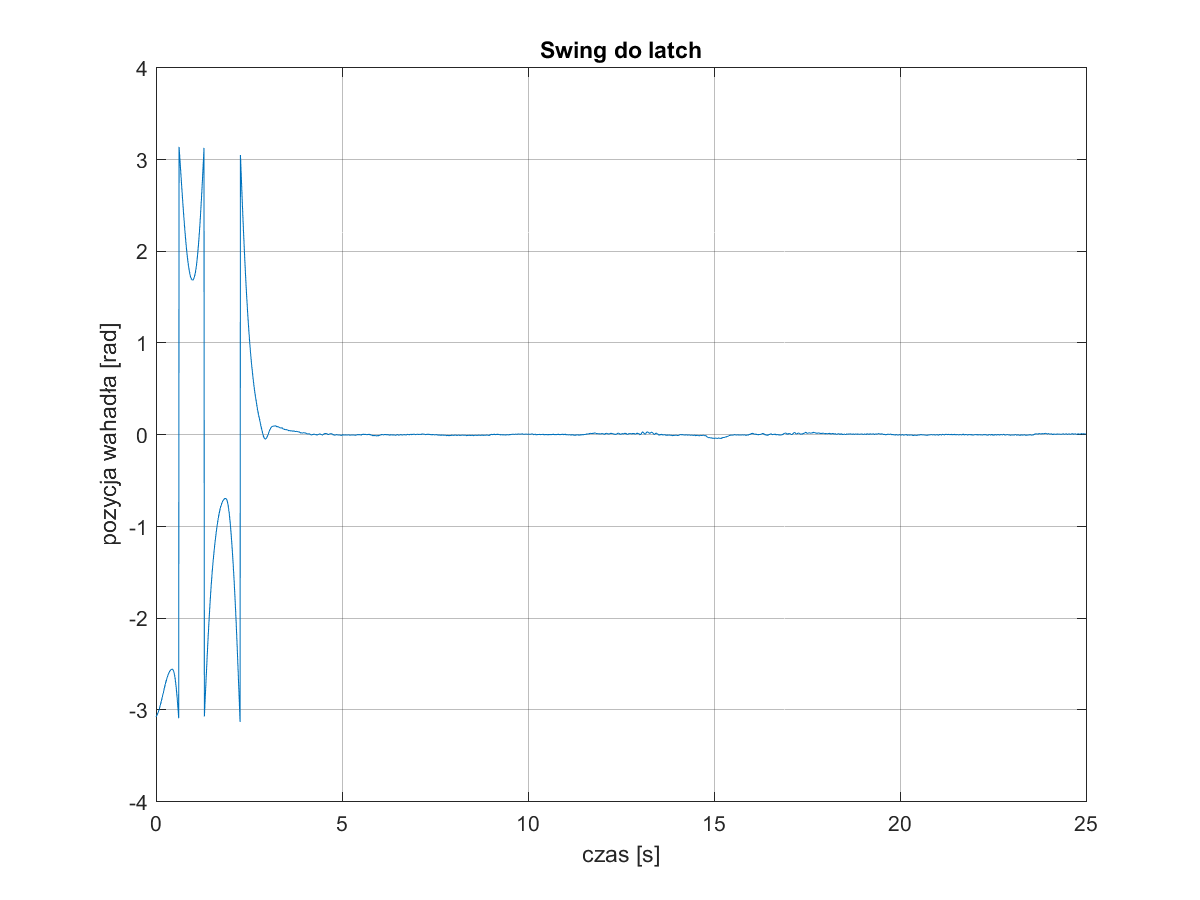
\includegraphics[width=3in]{obrazy/pendulum/Swing_do_latch_poz_wah.png}}
	~~
	\subfloat{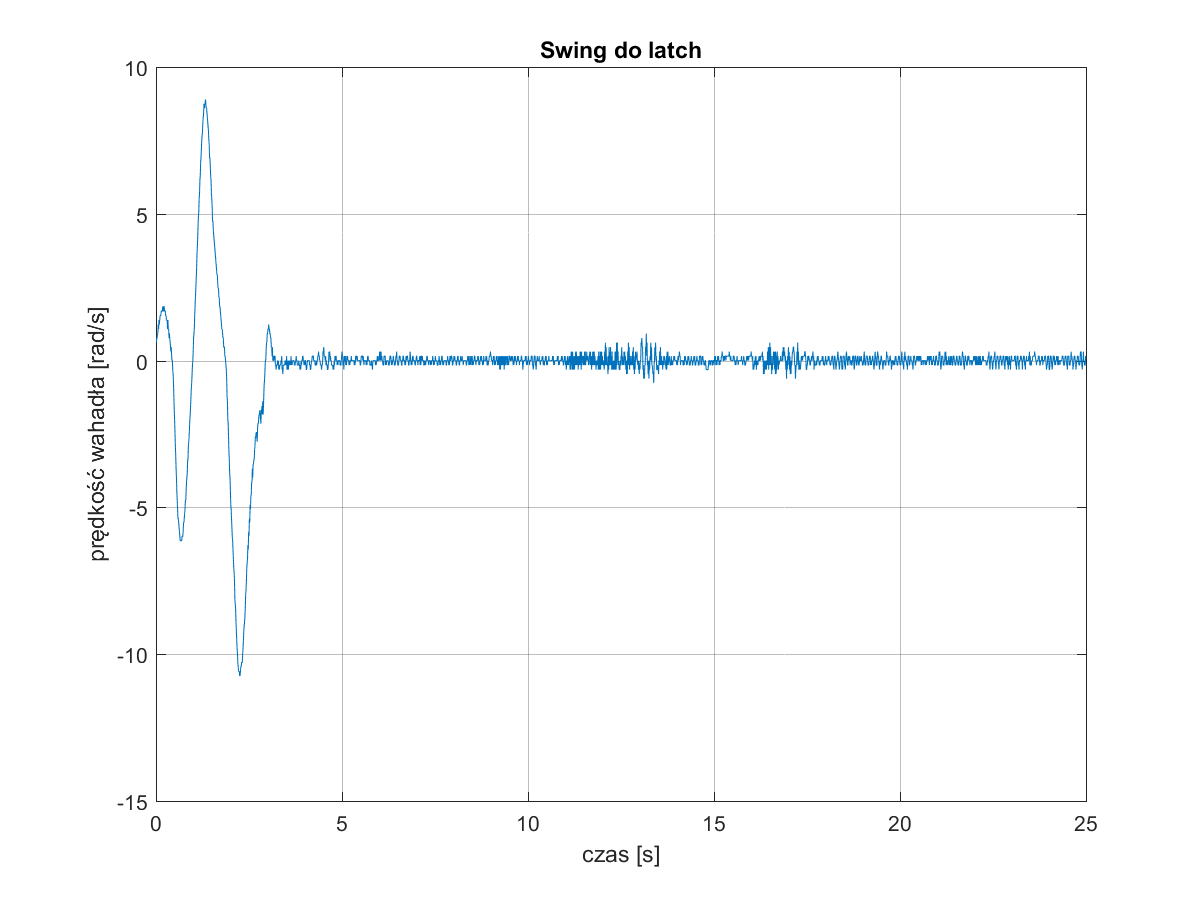
\includegraphics[width=3in]{obrazy/pendulum/Swing_do_latch_pred_wah.png}}
	
	\subfloat{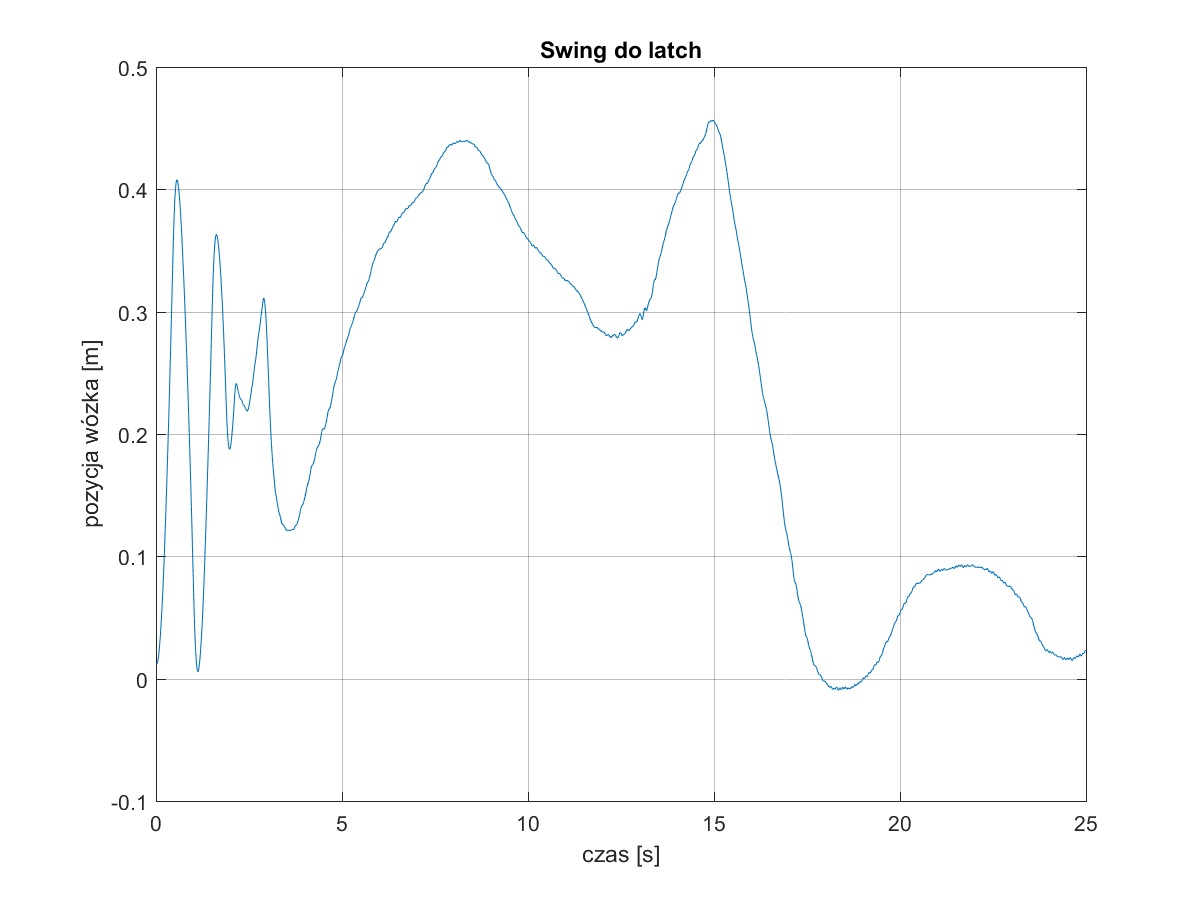
\includegraphics[width=3in]{obrazy/pendulum/Swing_do_latch_poz_woz.png}}
	~~
	\subfloat{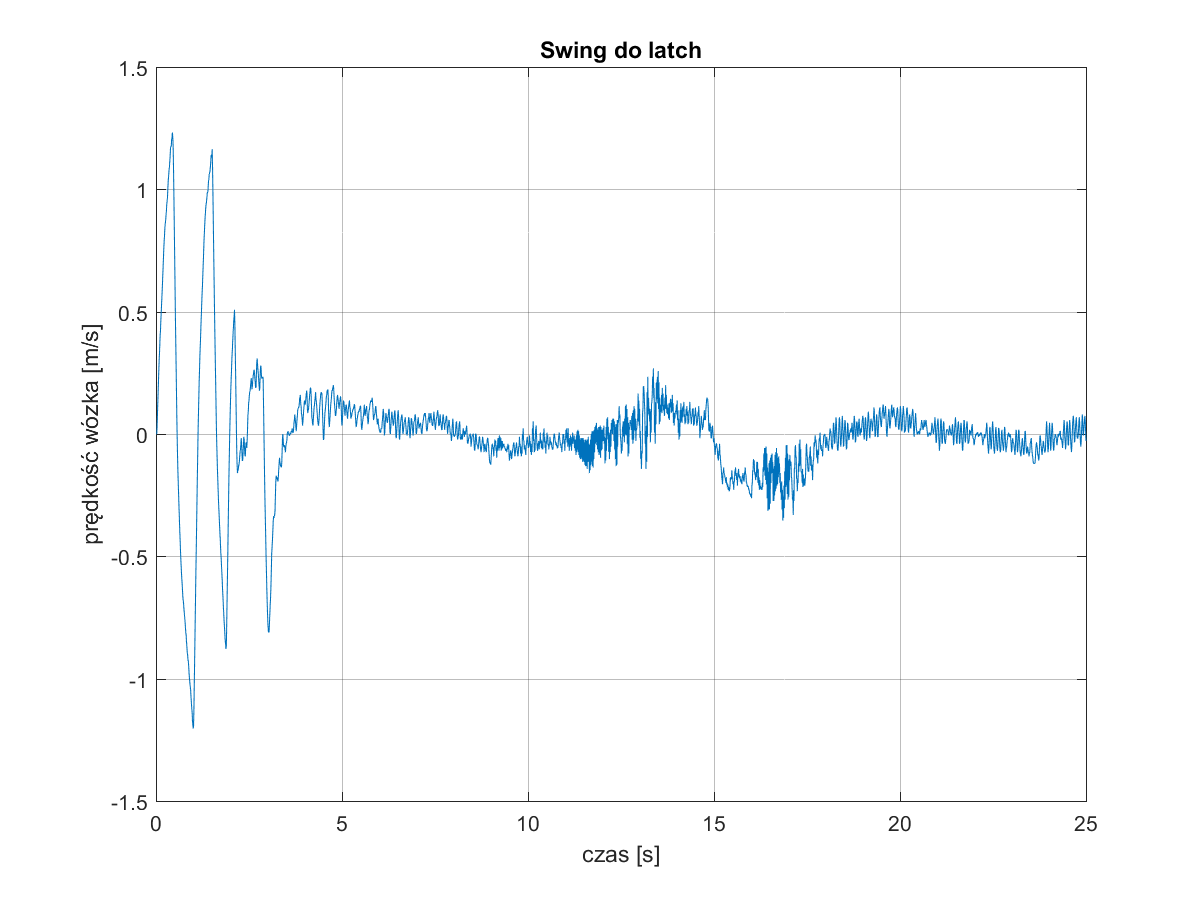
\includegraphics[width=3in]{obrazy/pendulum/Swing_do_latch_pred_woz.png}}
	
	\subfloat{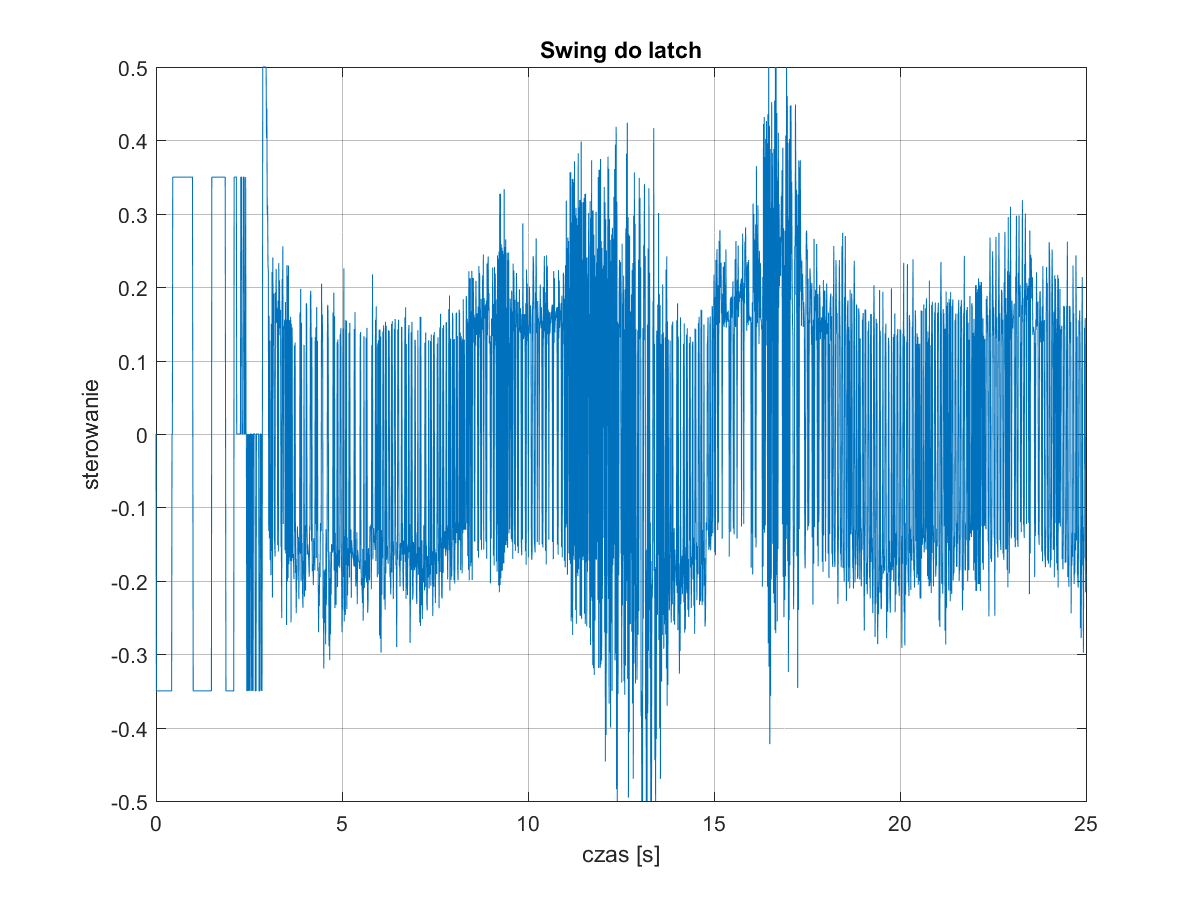
\includegraphics[width=3in]{obrazy/pendulum/Swing_do_latch_ster.png}}
%	~~
%	\subfloat{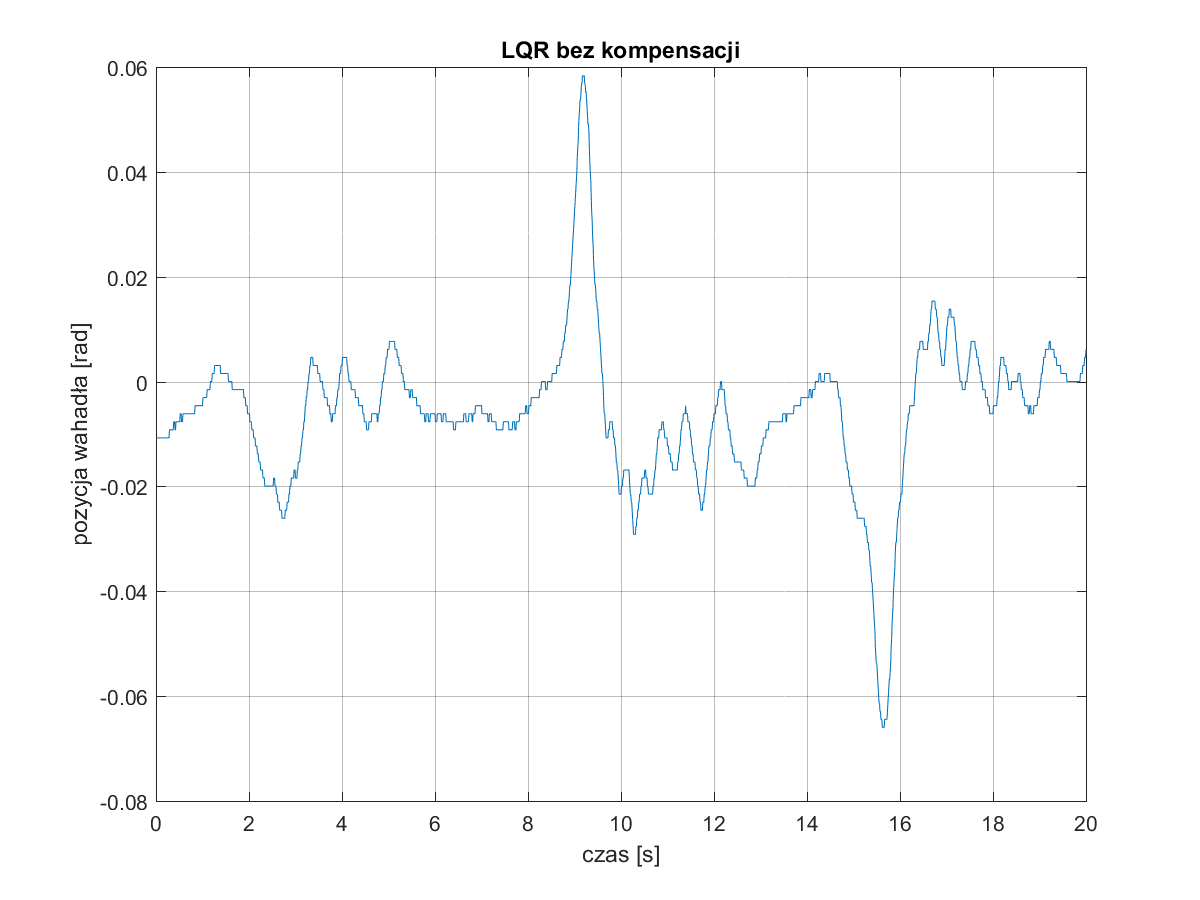
\includegraphics[width=2.8in]{obrazy/pendulum/LQR_bezk_poz_wah.png}}
	\caption{Swing-up wraz ze stabilizacją wahadła, zmiana referencyjnego położenia wózka.}
\label{fig:Swing1}
\end{figure}
